\mysection[WildStrawberry]{\centering Stetige Funktionen}
\mysubsection{Reellwertige Funktionen}
Sei $D$ eine beliebige Menge. Die Menge $R^D$ aller Funktionen $f:D\rightarrow \mathbb{R}$ bildet einen Vektorraum über $\mathbb{R}$, wobei Addition, skalare Multiplikation, und das Produkt gegeben sind durch: 
\begin{enumerate}
    \item $(f_1+f_2)(x)=f_1(x)+f_2(x)$
    \item $(\alpha \cdot f)(x)=\alpha \cdot f(x)$
    \item $(f_1\cdot f_2)(x)=f_1(x)f_2(x)$
\end{enumerate}
wobei $f_1,f_2,f\in\mathbb{R}^D,x\in D,\alpha\in\mathbb{R}$.

Eine konstante Funktion ist eine, die immer denselben Wert annimt. Darunter gibt es die Funktionen $\mathtt{0},\mathtt{1}\in\mathbb{R}^D$:
\begin{enumerate}
    \item $\mathtt{0}(x)=0\ \forall x\in D$
    \item $\mathtt{1}(x)=1\ \forall x\in D$
\end{enumerate}
Offensichtlich gilt $f+\mathtt{0}=f,g\cdot\mathtt{1}=g\ \forall f,g\in\mathbb{R}^D$. $\mathbb{R}^D$ versehen mit $+,\cdot$ erfüllt die Körperaxiome (ausser: falls $|D|\geq 2$ gibt es immer ein $f\not = \mathtt{0}$, das kein multiplikatives Inverses besitzt.

Auf $\mathbb{R}^D$ definieren wir eine Ordnung: $f\leq g \Leftrightarrow f(x)\leq g(x)\ \forall x\in D$. Weiter gilt $f$ ist nicht negativ $\Leftrightarrow \mathtt{0}\leq f$.

\DEF{Beschränktheit}{Sei $f\in\mathbb{R}^D$. Dann $f(D)=\{f(x)|x\in D\}$ und 
\begin{enumerate}
    \item $f$ ist nach oben beschränkt $\Leftrightarrow f(D)\subseteq\mathbb{R}$ ist nach oben beschränkt.
    \item $f$ ist nach unten beschränkt $\Leftrightarrow f(D)\subseteq\mathbb{R}$ ist nach unten beschränkt.
    \item $f$ ist beschränkt $\Leftrightarrow f(D)\subseteq\mathbb{R}$ ist beschränkt.
\end{enumerate}}

\DEF{Monotonie}{Sei $D\subseteq\mathbb{R}$. Eine Funktion $f:D\rightarrow\mathbb{R}$ ist
\begin{enumerate}
    \item monoton wachsend $\Leftrightarrow\ \forall x,y\in D: x\leq y \Rightarrow f(x)\leq f(y)$.
    \item streng monoton wachsend $\Leftrightarrow\ \forall x,y\in D: x<y\Rightarrow f(x)<f(y)$.
    \item monoton fallend $\Leftrightarrow\ \forall x,y\in D: x\leq y\Rightarrow f(x)\geq f(y)$.
    \item streng monoton fallend $\Leftrightarrow\ \forall x,y\in D: x<y\Rightarrow f(x)>f(y)$
    \item monoton $\Leftrightarrow (f$ ist monoton wachsend$) \lor (f$ ist monoton fallend$)$.
    \item streng monoton $\Leftrightarrow (f$ ist streng monoton wachsend$) \lor (f$ ist streng monoton fallend$)$.
\end{enumerate}}

\NOTE{3.1.3}{Sei $n\in\mathbb{N}$. Sei $f:\mathbb{R}\rightarrow\mathbb{R}$ definiert durch $x\mapsto x^n$. Dann $f$ (streng) monoton wachsend $\Leftrightarrow n\ mod\ 2 = 1$.}

\SA{}{Sei $f:[0,1]\rightarrow[0,\infty)$ monoton. Dann ist das Bild von $f$ immer ein beschränktes Intervall $[a,b]\subset[0,\infty)$ mit $0\leq a\leq b < \infty \Rightarrow f$ nicht surjektiv.}


\mysubsection{Stetigkeit}
\DEF{Stetigkeit in einem Punkt}{Sei $D\subseteq\mathbb{R},x_0\in D$. $f:D\rightarrow\mathbb{R}$ ist in $x_0$ stetig $\Leftrightarrow\ \forall\varepsilon > 0\ \exists\delta > 0:\forall x\in D\ (|x-x_0|<\delta\Rightarrow |f(x)-f(x_0)| < \varepsilon)$.}
\begin{figure}[H]
 \centering
 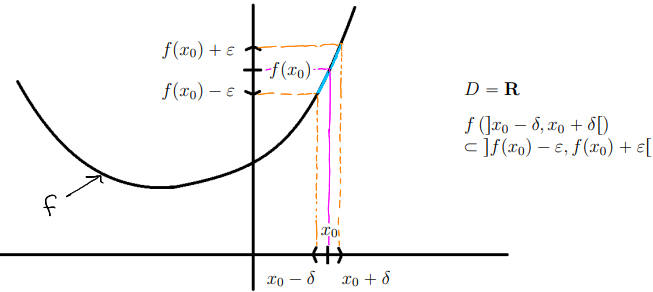
\includegraphics[width=\linewidth,keepaspectratio]{pictures/stetigkeit_in_einem_punkt.png} 
\end{figure}

\DEF{Stetigkeit einer Funktion}{$f:D\rightarrow\mathbb{R}$ ist stetig $\Leftrightarrow f$ ist in jedem Punkt $x\in D$ stetig.}

\SA{3.2.4 Folgenstetigkeit}{Sei $x_0\in D\subseteq\mathbb{R}$ und $f:D\rightarrow\mathbb{R}$ stetig in $x_0$ $\Leftrightarrow\ \forall (a_n)_{n\geq 1}\subseteq D: lim_{n\rightarrow\infty}a_n=x_0\Rightarrow lim_{n\rightarrow\infty}f(a_n)=f(x_0)$.}

\COR{3.2.5}{Sei $x_0\in D\subseteq\mathbb{R},\lambda\in\mathbb{R}$ und $f:D\rightarrow\mathbb{R},g:D\rightarrow\mathbb{R}$ beide stetig in $x_0$.

(1) Dann sind $f+g,\lambda\cdot f,f\cdot g$ stetig in $x_0$.

(2) Falls $g(x_0)\not = 0$ dann ist $\frac{f}{g}:D\cap\{x\in D:g(x)\not =0\}\rightarrow\mathbb{R}$ definiert durch $x\mapsto\frac{f(x)}{g(x)}$ stetig in $x_0$.}

\DEF{Polynomiale Funktion}{Eine polynomiale Funktion $P:\mathbb{R}\rightarrow\mathbb{R}$ ist eine Funktion der Form $P(x)=a_nx^n+...+a_0$ wobei $a_n,...,a_0\in\mathbb{R}$. Falls $a_n\not = 0$ ist $n$ der Grad von $P$.}

\COR{3.2.7}{Polynomiale Funktionen sind auf ganz $\mathbb{R}$ stetig.}

\COR{3.2.8}{Seien $P,Q$ polynomiale Funktionen auf $\mathbb{R}$ mit $Q\not =\mathtt{0}$. Seien $x_1,...,x_m$ die Nullstellen von $Q$. Dann ist $\frac{P}{Q}:\mathbb{R}\ \{x_1,...,x_m\}\rightarrow\mathbb{R}$ definiert duch $x\mapsto\frac{P(x)}{Q(x)}$ stetig.}

\mysubsection{Zwischenwertsatz}
Seien $x_1,x_2\in\mathbb{R}$. Dann liegt $c$ zwischen $x_1$ und $x_2 \Leftrightarrow (x_1\leq x_2 \land c\in[x_1,x_2]) \lor (x_2\leq x_1 \land c\in[x_2,x_1])$.

\SA{3.3.1 Bolzano 1817}{Sei $I\subseteq\mathbb{R}$ ein Intervall, $f:I\rightarrow\mathbb{R}$ eine stetige Funktion und $a,b\in I$. Dann $\forall c$ zwischen $f(a)$ und $f(b)$ gibt es ein $z$ zwischen $a$ und $b$ mit $f(z)=c$.}
\begin{figure}[H]
 \centering
 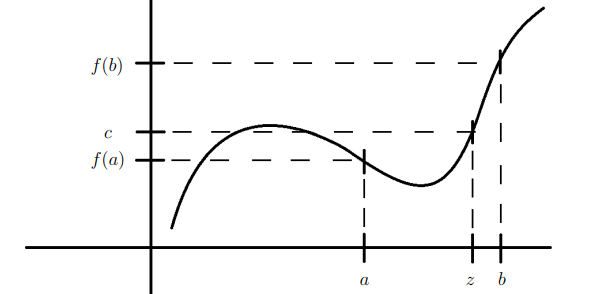
\includegraphics[width=\linewidth,keepaspectratio]{pictures/zwischenwertsatz.png} 
\end{figure}

\COR{3.3.2}{Sei $P(x)=a_nx^n+a_{n-1}x^{n-1}+...+a_0$ ein Polynom mit $a_n\not = 0$ und $n$ ungerade. Dann besitzt $P$ mindestens eine Nullstelle in $\mathbb{R}$.}

\mysubsection{Min-Max Satz}
\DEF{Kompakt}{Ein Intervall $I\subseteq\mathbb{R}$ ist kompakt, falls es von der Form $I=[a,b], a\leq b$ ist.}

\DEF{Notation}{Sei $D$ eine Menge und $f,g:D\rightarrow\mathbb{R}$.
\begin{itemize}
    \item $\forall x\in D: |f|(x):=|f(x)|$
    \item $\forall x\in D: max(f,g)(x):=max(f(x),g(x))$
    \item $\forall x\in D: min(f,g)(x):=min(f(x),g(x))$
\end{itemize}}

\LEM{3.4.3}{Sei $D\subseteq\mathbb{R},x_0\in D$ und $f,g:D\rightarrow\mathbb{R}$ stetig in $x_0$. Dann sind $|f|,max(f,g),min(f,g)$ stetig in $x_0$.}

\LEM{3.4.4}{Sei $(x_n)_{n\geq 1}$ eine konvergente Folge in $\mathbb{R}$ mit $lim_{n\rightarrow\infty}X_n\in\mathbb{R}$. Sei $a\leq b$. Falls $\{x_n:n\geq 1\}\subseteq[a,b] \Rightarrow lim_{n\rightarrow\infty}x_n\in[a,b]$.}

\SA{3.4.5}{Sei $I=[a,b]$. Sei $f:I\rightarrow\mathbb{R}$ stetig. Dann $\exists u,v\in I: f(u)\leq f(x)\leq f(v)\ \forall x\in I \Leftrightarrow f$ ist beschränkt.}

\mysubsection{Satz der Umkehrabbildung}
\SA{3.5.1}{Seien $D_1,D_2\subseteq\mathbb{R}$, $f:D_1\rightarrow D_2,$ $g:D_2\rightarrow\mathbb{R},$ $x_0\in D_1$. Dann $f$ in $x_0$ und $g$ in $f(x_0)$ stetig $\Leftrightarrow g\circ f:D_1\rightarrow\mathbb{R}$ in $x_0$ stetig. }

\COR{3.5.2}{Falls $f$ auf $D_1$ und $g$ auf $D_2$ stetig $\Rightarrow g\circ f$ auf $D_1$ stetig.}

\SA{3.5.3}{Sei $I\subseteq\mathbb{R}$ ein Intervall und $f:I\rightarrow\mathbb{R}$ stetig, streng monoton. Dann ist $J:=f(i)\subseteq\mathbb{R}$ ein Intervall und $f^{-1}:J\rightarrow I$ ist stetig, streng monoton.}

\mysubsection{Reelle Exponentialfunktion}
\SA{3.6.1}{$exp:\mathbb{R}\rightarrow(0,\infty)$ ist stetig, streng monoton wachsend, und surjektiv.}

\DEF{Natürlicher Logarithmus}{Die Umkehrabbildung von $exp:\mathbb{R}\rightarrow(0,\infty)$ ist der natürliche Logarithmus $ln:(0,\infty)\rightarrow\mathbb{R}$.}

\COR{3.6.5}{$ln:(0,\infty)\rightarrow\mathbb{R}$ ist stetig, streng monoton wachsend, und bijektiv.}

\COR{3.6.6}{
\begin{enumerate}
    \item Für $a>0$ ist $(0,\infty)\rightarrow(0, \infty), x\mapsto x^a$ stetig, streng monoton wachsend, und bijektiv.
    \item Für $a < 0$ ist $(0,\infty)\rightarrow(0, \infty), x\mapsto x^a$ stetig, streng monoton fallend, und bijektiv.
\end{enumerate}}

\mysubsection{Konvergenz von Funktionenfolgen}
Sei $D$ eine Menge. Eine (reellwertige) Funktionenfolge ist eine Abbildung $\mathbb{N}\rightarrow\mathbb{R}^D,n\mapsto f_n$. D.h. jedes $f_n$ ist eine Funktion $D\rightarrow\mathbb{R}$.

Für eine Funktionenfolge schreiben wir $(f_n)_{n\geq 0}$. $\forall x\in D$ erhalten wir eine Folge $(f_n(x))_{n\geq 0}$ in $\mathbb{R}$.

\DEF{Punktweise Konvergenz}{Die Funktionenfolge $(f_n)_{n\geq 0}$ konvergiert punktweise gegen $f:D\rightarrow\mathbb{R}$, falls $\forall x\in D:lim_{n\rightarrow\infty}f_n(x)=f(x)$ $\Leftrightarrow$ $\forall x\in D\ \forall\varepsilon > 0\ \exists N\in\mathbb{N}\ \forall n\geq N: |f_n(x)-f(x)|<\varepsilon$. $f$ ist nicht zwingend in $D$ stetig.}

\DEF{Gleichmässige Konvergenz}{Die Funktionenfolge $f_n:D\rightarrow\mathbb{R}$ konvergiert gleichmässig in $D$ gegen $f:D\rightarrow\mathbb{R}$, falls $\forall\epsilon > 0$ $\exists N\in\mathbb{N}$ s.d. $\forall n\geq N,\forall x\in D: |f_n(x)-f(x)|<\epsilon$ $\Leftrightarrow f_n$ liegt komplett im $\epsilon$-Schlauch um $f$.}

\SA{3.7.4}{Sei $D\subseteq\mathbb{R}$ und $f_n:D\rightarrow\mathbb{R}$ eine Funktionenfolge bestehend aus (in $D$) stetigen Funktionen die (in $D$) gleichmässig gegen $f:D\rightarrow\mathbb{R}$ konvergieren. Falls $f_n$ $\forall n\geq 1$ stetig in $x_0\in D \Rightarrow f$ stetig in $x_0$.}

\COR{3.7.6 Cauchy Kriterium}{Die Funktionenfolge $f_n:D\rightarrow\mathbb{R}$ konvergiert gleichmässig in $D$ $\Leftrightarrow$ $\forall\varepsilon > 0\ \exists N\geq 1:$ $\forall n,m\geq N\ \forall x\in D:$ $ |f_n(x)-f_m(x)|<\varepsilon$.}

\COR{3.7.7}{Sei $D\subseteq\mathbb{R}$. Falls $f_n:D\rightarrow\mathbb{R}$ gleichmässig konvergente Folge stetiger Funktionen $\Rightarrow f(x):=lim_{n\rightarrow\infty}f_n(x)$ stetig.}

\mysubsection{Reihen von Funktionen}
\DEF{Konvergenz}{Die Reihe $\sum_{k=0}^{\infty}f_k(x)$ konvergiert punktweise (resp. gleichmässig) in $D$, falls die Funktionenfolge $S_n(x):=\sum_{k=0}^nf_k(x)$ punktweise (resp. gleichmässig) konvergiert.}

\SA{3.7.9}{Sei $D\subseteq\mathbb{R}$ und $f_n:D\rightarrow\mathbb{R}$ eine Funktionenfolge. Sei $|f_n(x)|\leq c_n\in[0,\infty)\ \forall x\in D$ und $\sum_{n=0}^{\infty}c_n$ konvergent. Dann konvergiert $\sum_{n=0}^{\infty}f_n(x)$ gleichmässig in $D$. Falls alle $f_n$ in $D$ stetig sind, dann ist $f(x):=\sum_{n=0}^{\infty}f_n(x)$ eine in $D$ stetige Funktion.}

\SA{3.7.11}{Sei $\sum_{k=0}^{\infty}c_kx^k$ eine Potenzreihe mit $\rho > 0$. Sei $f(x):=\sum_{k=0}^{\infty}c_kx^k,\ |x|<\rho$. Dann gilt $\forall 0\leq r < \rho$ konvergiert $\sum_{k=0}^{\infty}c_kx^k$ gleichmässig auf $[-r,r]$ und $f:(-\rho,\rho)\rightarrow\mathbb{R}$ stetig.}


\mysubsection{Trigonometrische Funktionen}
\DEF{Sinus}{Sei $z\in\mathbb{C}$. $sin(z) = z-\frac{z^3}{3!}+\frac{z^5}{5!}-\frac{z^7}{7!}+...=\sum_{n=0}^{\infty}\frac{(-1)^nz^{2n+1}}{(2n+1)!}$.}

\DEF{Cosinus}{Sei $z\in\mathbb{C}$. $cos(z) = 1-\frac{z^2}{2!}+\frac{z^4}{4!}-\frac{z^6}{6!}+...=\sum_{n=0}^{\infty}\frac{(-1)^nz^{2n}}{(2n)!}$.}

\DEF{Tangens}{$tan(z)=\frac{sin(z)}{cos(z)}, z\not\in\frac{\pi}{2}+\pi\cdot\mathbb{Z}$.}

\DEF{Cotangens}{$cot(z)=\frac{cos(z)}{sin(z)}, z\not\in\pi\cdot\mathbb{Z}$.}

\DEF{Arcsin}{$arcsin:[-1,1]\rightarrow[-\frac{\pi}{2},\frac{\pi}{2}]$ ist die Umkehrfunktion von $sin:[-\frac{\pi}{2},\frac{\pi}{2}]\rightarrow[-1,1]$. Also $arcsin:=sin^{-1}$.}

\DEF{Arccos}{$arccos:[-1,1]\rightarrow[0,\pi]$ ist die Umkehrfunktion von $cos:[0,\pi]\rightarrow[-1,1]$. Also $arccos:=cos^{1}$.}

\DEF{Arctan}{$arctan:(-\infty, \infty)\rightarrow (-\frac{\pi}{2},\frac{\pi}{2})$ ist die Umkehrfunktion von $tan:(-\frac{\pi}{2},\frac{\pi}{2})\rightarrow(-\infty, \infty)$. Also $arctan:=tan^{-1}$. $arctan(0)=0, arctan(1)=\frac{\pi}{4}$, $\lim_{x\rightarrow\infty}arctan(x)=\frac{\pi}{2}$, $\lim_{x\rightarrow-\infty}arctan(x)=\frac{-\pi}{2}$.}

\DEF{Arccot}{$arccot:(-\infty, \infty)\rightarrow (0,\pi)$ ist die Umkehrfunktion von $cot:(0,\pi)\rightarrow(-\infty,\infty)$. Also $arccot:=cot^{-1}$.}

\NOTE{}{Für $x\in\mathbb{R}$ ist $cos(x)=Re(exp(ix))$, $sin(x)=Im(exp(ix))$.}

\NOTE{}{Die Reihen $sin(z)$ und $cos(z)$ konvergieren absolut $\forall z\in\mathbb{C}$. Konvergenzradius ist also in beiden Fällen $\infty$.}

\SA{3.8.1}{$sin:\mathbb{R}\rightarrow\mathbb{R}$ und $cos:\mathbb{R}\rightarrow\mathbb{R}$ sind stetig.}

\SA{3.8.2}{
\begin{enumerate}
    \item $exp(iz)=cos(z)+isin(z)\ \forall z\in\mathbb{C}$
    \item $cos(z)=cos(-z)$ und $sin(-z)=-sin(z)\ \forall z\in\mathbb{C}$
    \item $sin(z)=\frac{e^{iz}-e^{-iz}}{2i}$,\  $cos(z)=\frac{e^{iz}+e^{-iz}}{2}$
    \item $sin(z+w)=sin(z)cos(w)+cos(z)sin(w)$\\ $cos(z+w)=cos(z)cos(w)-sin(z)sin(w)$
    \item $cos(z)^2+sin(z)^2=1\ \forall z\in\mathbb{C}$
    \item $sin(z) - sin(w) = 2sin(\frac{z-w}{2})cos(\frac{z+w}{2})$ $cos(z)-cos(w)=-2sin(\frac{z-w}{2})sin(\frac{z+w}{2})$
\end{enumerate}}

\COR{3.8.3 (Winkelverdopplungsformeln)}{
\begin{enumerate}
    \item $sin(2z)=2sin(z)cos(z)$
    \item $cos(2z)=cos(z)^2-sin(z)^2$
    \item $cos(2z)=1-2sin(z)^2\Leftrightarrow sin(z)^2=\frac{1}{2}-\frac{cos(2z)}{2}$.
    \item $cos(z)^2=\frac{cos(2z)}{2}+\frac{1}{2}$.
\end{enumerate}}

\mysubsection{Die Kreiszahl $\pi$}
\SA{3.9.1}{$sin(x)$ hat auf $(0,\infty)$ mindestens eine Nullstelle. Sei $\pi=inf\{t:t>0,sin(t)=0\}$ die erste Nullstelle. Dann gilt:
\begin{enumerate}
    \item $sin(\pi)=0$, $\pi\in(2,4)$.
    \item $\forall x\in (0,\pi):sin(x)>0$.
    \item $e^{\frac{i\pi}{2}}=i$.
\end{enumerate}}

\COR{3.9.2}{$x\geq sin(x) \geq x-\frac{x^3}{3!}\ \forall 0 \leq x \leq \sqrt{6}$.}

\COR{3.9.3}{
\begin{enumerate}
    \item $e^{i\pi}=-1,\ e^{i2\pi}=1$
    \item $sin(x+\frac{\pi}{2})=cos(x),cos(x+\frac{\pi}{2})=-sin(x)\ \forall x\in\mathbb{R}.$
    \item $sin(x+\pi)=-sin(x), sin(x+2\pi)=sin(x)\ \forall x\in\mathbb{R}$.
    \item $cos(x+\pi)=-cos(x), cos(x+2\pi)=cos(x)\ \forall x\in\mathbb{R}$.
    \item $\{x:sin(x)=0\}=\{k\cdot\pi:k\in\mathbb{Z}\}$.\\
            $sin(x)>0\ \forall x\in(2k\pi,(2k+1)\pi),\  k\in\mathbb{Z}$.\\
            $sin(x)<0\ \forall x\in((2k+1)\pi, (2k+2)\pi),\  k\in\mathbb{Z}$.
    \item $\{x:cos(x)=0\}=\{k\cdot\pi+\frac{\pi}{2}:k\in\mathbb{Z}\}$.\\
            $cos(x)>0\ \forall x\in(2k\pi-\frac{\pi}{2},(2k+1)\pi-\frac{\pi}{2}),\  k\in\mathbb{Z}$.\\
            $cos(x)<0\ \forall x\in((2k+1)\pi-\frac{\pi}{2}, (2k+2)\pi-\frac{\pi}{2}),\  k\in\mathbb{Z}$.
\end{enumerate}}

\DEF{Komplexer Einheitskreis}{Sei $S^1=\{z\in\mathbb{C}:|z|=1\}$ der komplexe Einheitskreis. Dann $cis:[0,2\pi)\rightarrow S^1,x\mapsto e^{ix}$ bijektiv.}

\DEF{Bogenmass}{Sei $x\in\mathbb{R},n\in\mathbb{N}^*,z_{n,k}:=e^{\frac{ikx}{n}}\in S^1$ für $0\leq k\leq n$. Dann ist $L_n:=\sum_{k=1}^n|z_{n,k}-z_{n,k-1}|=n|z_{n,1}-z_{n,0}|=n\cdot 2|sin(\frac{x}{2n})|$ die Länge des Polygonzuges $z_{n,0},z_{n,1},...,z_{n,n}$ und es gilt $lim_{n\rightarrow\infty}=|x|$.}

\begin{figure}[H]
 \centering
 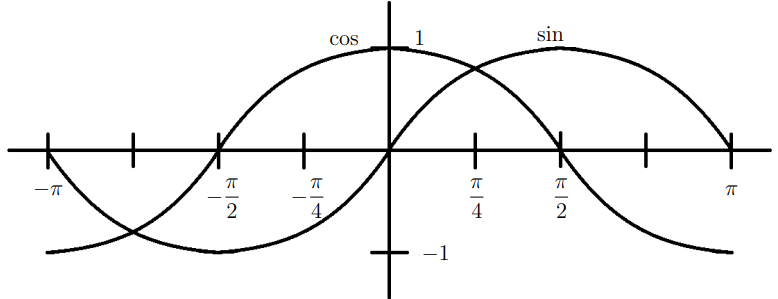
\includegraphics[width=\linewidth,keepaspectratio]{pictures/sinus_cosinus.png} 
\end{figure}

\begin{figure}[H]
 \centering
 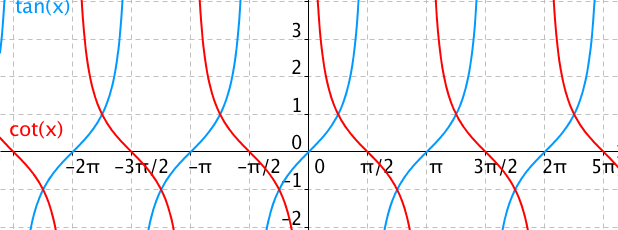
\includegraphics[width=\linewidth,keepaspectratio]{pictures/tan_cot.png} 
\end{figure}

\mysubsection{Hyperbel und Areafunktionen}
\DEF{Cosinus Hyperbolicus}{$cosh(x)=\frac{e^x+e^{-x}}{2}$.}

\DEF{Sinus Hyperbolicus}{$sinh(x)=\frac{e^x-e^{-x}}{2}$.}

\DEF{Tangens Hyperbolicus}{$tanh(x)=\frac{sinh(x)}{cosh(x)}=\frac{e^x-e^{-x}}{e^x+e^{-x}}$.}

\DEF{Arcosh}{$arcosh:[1,\infty)\rightarrow[0,\infty)$ bezeichnet die Umkehrfunktion von $cosh:[0,\infty)\rightarrow[1,\infty)$. Also $arcosh:=cosh^{-1}$.}

\DEF{Arsinh}{$arsinh:\mathbb{R}\rightarrow\mathbb{R}$ bezeichnet die Umkehrfunktion von $sinh:\mathbb{R}\rightarrow\mathbb{R}$. Also $arsinh:=sinh^{-1}$.}

\DEF{Artanh}{$artanh:(-1,1)\rightarrow\mathbb{R}$ bezeichnet die Umkehrfunktion von $tanh:\mathbb{R}\rightarrow(-1,1)$. Also $artanh:=tanh^{-1}$.}

\SA{}{
\begin{enumerate}
    \item $cosh^2(x)-sinh^2(x)=1\ \forall x\in\mathbb{R}$.
    \item $cosh(2x)=cosh^2(x)+sinh^2(x)$.
    \item $sinh(2x)=2sinh(x)cosh(x)$.
\end{enumerate}}

\begin{figure}[H]
 \centering
 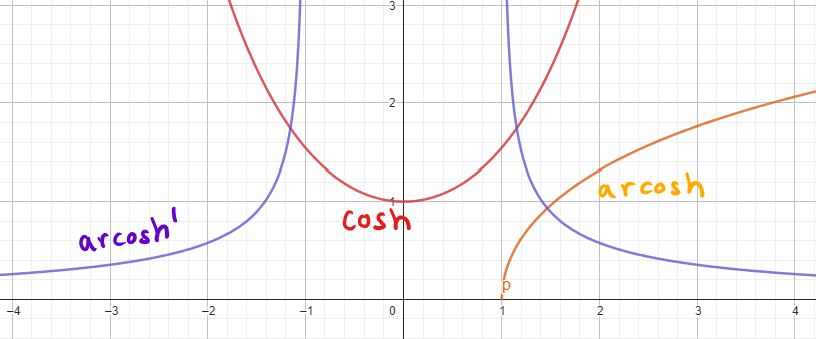
\includegraphics[width=\linewidth,keepaspectratio]{pictures/hyperbolic_cosinus.png} 
\end{figure}

\begin{figure}[H]
 \centering
 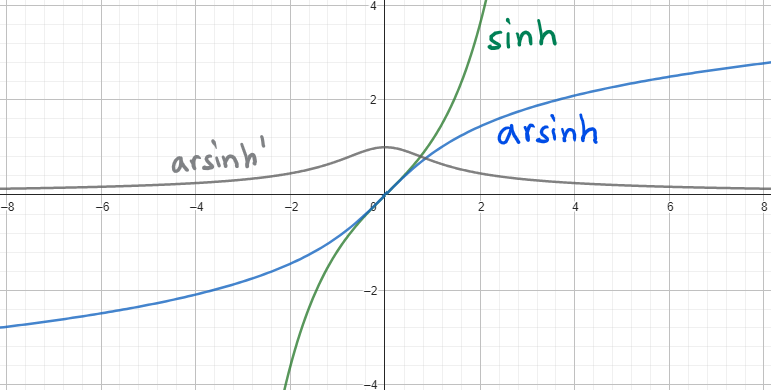
\includegraphics[width=\linewidth,keepaspectratio]{pictures/hyperbolic_sinus.png} 
\end{figure}

\mysubsection{Grenzwerte von Funktionen}
\DEF{Häufungspunkt}{Sei $D\subseteq\mathbb{R}$. Ein Häufungspunkt von $D$ ist eine Zahl $x_0\in\mathbb{R}$ oder $x_0=\infty$ oder $x_0=-\infty$ s.d. $\exists (a_n)_{n\geq 1}$ in $D\setminus \{x_0\}$ mit $lim_{n\rightarrow\infty}a_n=x_0$.

Umformulierungen:
\begin{itemize}
    \item Fall $x_0\in\mathbb{R}:$ $\forall\delta > 0:((x_0-\delta,x_0+\delta)\setminus \{x_0\})\cap D\not=\emptyset$.
    \item Fall $x_0=\infty:$ $\forall c>0: (c,\infty)\cap D\not=\emptyset$.
    \item Fall $x=-\infty:$ $\forall c>0: (-\infty,-c)\cap D\not = \emptyset$.
\end{itemize}}

\EXAMPLE{3.10.2}{Sei $D=\{0\}\cup(1,2)$. Dann ist $D'=[1,2]$ die Menge aller Häufungspunkte von $D$ und $0$ ist ein isolierter Punkt von $D$.}

\DEF{Existenz des Grenzwerts}{Sei $f:D\rightarrow\mathbb{R}$, $x_0$ ein Häufungspunkt von $D$, $A\in\mathbb{R}$ oder $A=\infty$ oder $A=-\infty$. Dann $lim_{x\rightarrow x_0}f(x)=A$ $\Leftrightarrow$ $\forall (a_n)_{n\geq 1}$ in $D\setminus\{x_0\}:$ $(lim_{n\rightarrow\infty}a_n=x_0 \Rightarrow lim_{n\rightarrow\infty}f(a_n)=A)$.

Falls kein solches $A$ existiert, sagen wir, der Grenzwert von $f$ für $x\rightarrow x_0$ existiert nicht.

Umformulierungen:
\begin{enumerate}
    \item Fall $x\in\mathbb{R}$ und $A\in\mathbb{R}$\\
            $lim_{x\rightarrow x_0}f(x)=A$ $\Leftrightarrow$ $\forall\varepsilon >0\ \exists\delta >0:\forall x\in ((x_0-\delta,x_0+\delta)\setminus \{x_0\})\cap D: |f(x)-A| < \varepsilon$.
    \item Fall $x\in\mathbb{R}$ und $A=-\infty$
            $lim_{x\rightarrow x_0}f(x)=A$ $\Leftrightarrow$ $\forall c >0\ \exists\delta >0:\forall x\in ((x_0-\delta,x_0+\delta)\setminus \{x_0\})\cap D: f(x) < -c$.
    \item Fall $x=-\infty$ und $A\in\mathbb{R}$
            $lim_{x\rightarrow x_0}f(x)=A$ $\Leftrightarrow$ $\forall\varepsilon >0\ \exists N >0:\forall x < -N, x\in D: |f(x)-A| < \varepsilon$.
    \item[...] Es gibt noch $6$ weitere Umformulierungen nach dem selben Schema.
\end{enumerate}}

\NOTE{3.10.4.2}{Sei $x_0\in D$. Dann $f$ stetig in $x_0$ $\Leftrightarrow lim_{x\rightarrow x_0}f(x)=f(x_0)$.}

\EXAMPLE{}{Sei $f:[0,2]\rightarrow\mathbb{R}$, $f(x)=\begin{cases}
    0 & x\in[0,1)\cup (1,2],\\
    1 & x=1.
\end{cases}$ Dann ist $lim_{x\rightarrow 1}f(x)=0\not = f(1)=1$ und $f$ ist nicht stetig in $x_0$. Merke: Wenn $x_0\not\in D$, dann kann $f:D\rightarrow\mathbb{R}$ in diesem Punkt nicht stetig sein.}

\DEF{Stetige Fortsetzung einer Funktion}{Wenn $x_0\not\in D$ und $lim_{x\rightarrow x_0}f(X)$ in $\mathbb{R}$ existiert, dann ist $f^{\sim}=\begin{cases}
    f(x) & x\in D,\\
    lim_{x\rightarrow x_0}f(x) & x=x_0
\end{cases}$ die stetige Fortsetzung von $f$, welche stetig in $x_0$ ist.}

\NOTE{3.10.4.3-5}{
\begin{enumerate}
    \item Sei $f,g:D\rightarrow\mathbb{R}$ und $lim_{x\rightarrow x_0}f(x),lim_{x\rightarrow x_0}g(x)$ existieren. Dann \begin{itemize}
    \item $lim_{x\rightarrow x_0}(f+g)(x)=lim_{x\rightarrow x_0}f(x)+lim_{x\rightarrow x_0}g(x)$.
    \item $lim_{x\rightarrow x_0}(f\cdot g)(x)=lim_{x\rightarrow x_0}f(x) \cdot lim_{x\rightarrow x_0}g(x)$.
    \end{itemize}
    \item Sei $f,g:D\rightarrow\mathbb{R}$, $f\leq g$, und beide Grenzwerte existieren. Dann $lim_{x\rightarrow x_0}f(x)\leq lim_{x\rightarrow x_0}g(x)$.
    \item Falls $g_1\leq f \leq g_2$ und $lim_{x\rightarrow x_0}g_1(x)=lim_{x\rightarrow x_0}g_2(x)$. Dann $\exists lim_{x\rightarrow x_0}f(x)$ und $lim_{x\rightarrow x_0}f(x)=lim_{x\rightarrow x_0}g_1(x)$.
\end{enumerate}}

\SA{3.10.6}{Seien $D,E\subseteq\mathbb{R}$, $x_0$ Häufungspunkt von $D$, $f:D\rightarrow E$. Angenommen $y_0:=lim_{x\rightarrow x_0}f(x)$ existiert und $y_0\in E$. $g:E\rightarrow\mathbb{R}$ stetig in $y_0$ $\Rightarrow lim_{x\rightarrow x_0}g(f(x))=g(y_0)$.}

\mysubsection{Links- und Rechtsseitige Grenzwerte}
\DEF{Rechtsseitiger Häufungspunkt und Grenzwert}{Sei $f:D\rightarrow\mathbb{R}$, $x_0\in\mathbb{R}$ ein Häufungspunkt von $D\cap(x_0,\infty)$. Dann ist $x_0$ ein rechtsseitiger Häufungspunkt.

Falls der Grenzwert von $f|_{D\cap[x_0,\infty)}$ für $x\rightarrow x_0$ existiert, wird er mit $lim_{x\rightarrow x_0^+}f(x)$ bezeichnet und nennt sich rechtsseitiger Grenzwert von $f$ bei $x_0$.

Falls $\forall\varepsilon > 0\ \exists\delta > 0: \forall x\in (x_0,x_0+\delta)\cap D: f(x) > \frac{1}{\varepsilon}$ $\Rightarrow lim_{x\rightarrow x_0^+}f(x)=\infty$.}


\DEF{Linksseitiger Häufungspunkt und Grenzwert}{Sei $f:D\rightarrow\mathbb{R}$, $x_0\in\mathbb{R}$ ein Häufungspunkt von $D\cap(-\infty, x_0)$. Dann ist $x_0$ ein linksseitiger Häufungspunkt.

Falls der Grenzwert von $f|_{D\cap(-\infty,x_0]}$ für $x\rightarrow x_0$ existiert, wird er mit $lim_{x\rightarrow x_0^-}f(x)$ bezeichnet und nennt sich linksseitiger Grenzwert von $f$ bei $x_0$.

Falls $\forall\varepsilon > 0\ \exists\delta > 0: \forall x\in (x_0,x_0+\delta)\cap D: f(x) < -\frac{1}{\varepsilon}$ $\Rightarrow lim_{x\rightarrow x_0^-}f(x)=\infty$.}

\SA{}{Sei $D\subseteq\mathbb{R},f:D\rightarrow\mathbb{R}$ und $x_0$ ein links- und rechtsseitiger Häufungspunkt von $D$. Dann $\exists\ lim_{x\rightarrow x_0}f(x)\Leftrightarrow(\exists\ lim_{x\rightarrow x_0^+}f(x) \land\exists\ lim_{x\rightarrow x_0^-}f(x)\land lim_{x\rightarrow x_0^+}f(x)=lim_{x\rightarrow x_0^-}f(x))$.}







